\section*{Источники и решения}

\subsection*{Любовь в Клептопии}

Эта головоломка появляется в книге Саймона Сингха \cite{} и была передана мне Кэролайн Калдербэнк, молодой дочерью математиков Ингрид Добеки и Роба Калдербэнка.
В решении, которое она имела в виду, Ян отправляет Марии коробку с кольцом в ней и одним из его замков на ней. По получении Мария прикрепляет свой собственный замок к коробке и отправляет ее обратно с обоими замками на ней.
Когда Ян получает ее, он снимает свой замок и отправляет коробку обратно Марии; вуаля!

Это решение не просто игра;
идея является фундаментальной в обмене ключами Диффи-Хеллмана, историческим прорывом в криптографии.

В зависимости от предположений, возможны и другие решения.
Мое любимое было предложено компанией участников конференции
«Ga\-the\-ring for Gardner VII», включая оригамиста Роберта Лэнга.
Для этого Ян должен найти замок, ключ которого имеет большое отверстие, или по крайней мере, отверстие, которое может быть достаточно увеличено сверлением, чтобы ключ мог быть нацеплен за душку другого замка.
Ян использует этот второй замок, с упомянутым ключом на его дужке, чтобы запереть маленькую пустую коробку, которую он отправляет Марии.
Когда пройдет достаточно времени для того, чтобы она получила ее (возможно, он ожидает электронного подтверждения от Марии), он отправляет кольцо в другой коробке, запертый первым замком.
Когда Мария получает коробку с кольцом, она поднимает всю первую коробку и использует ключ, прикрепленный к ней, чтобы получить доступ к своему кольцу.

\subsection*{Черви и вода}

Это скорее инженерная головоломка, чем математическая.
Она пришла ко мне от Балинта Вирага из Массачусетского технологического института.

Лори действительно может защититься от червей свесив с потолка большой навес, выходящий далеко за кровать.
Но навес должен загибаться внутрь под себя по краям, создавая кольцевой жёлоб, заполненный водой.
(См. Рисунок 2 для поперечного разреза навеса.)

\begin{figure}[h!]
\centering
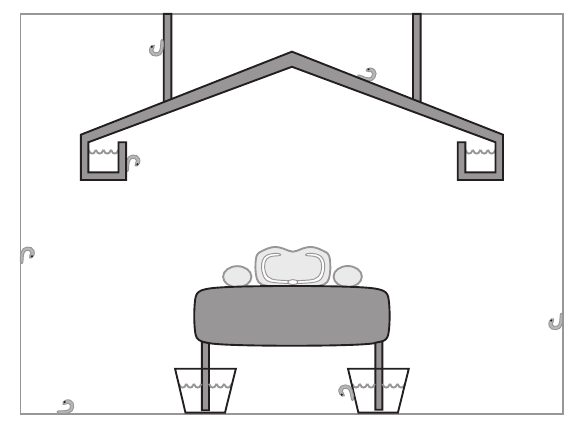
\includegraphics[scale=0.5]{pics/chervi}
\caption{Вертикальное сечение Лори в её защищенной от червей кровати.}
\end{figure}

Если у червей нет способа проникнуть в ее спальню сверху, Лори может выполнить ту же задачу, обведя комнату по краю жёлобом с водой.

\subsection*{Инспектор страусиных яиц}

Вариант этой увлекательной задачи появился в замечательной книге Джозефа Д. Э. Конхаузера, Дэна Веллмана и Стэна Вагона \cite{}.

Часто полезно считать данное число (в нашем случае 102???) переменной, даже если в конечном итоге нам интересно только одно значение.
Пусть $f(k)$ --- максимальное число этажей, которые можно проверить не более чем за $k$ бросков, имея в начале два яйца.
Таким образом, $f(1) = 1$ (прочность яйца может быть $0$ или $1$).
Предположим, что Оскару разрешено сделать $k$ бросков, и он делает первый с $n$-го этажа.
Если яйцо разбилось, то Оскару придётся бросить единственное оставшееся яйцо с 1-го этажа, затем с 2-го и так далее до $(n-1)$-го в худшем случае;
так что $n = k$ это лучшее, что возможно.
Если яйцо пережило падение с $k$-го этажа, то ему придётся проверить все этажи выше оставшимися $k-1$ броском (используя два яйца).
Следовательно, $f(k - 1) + k$ это максимальное число этажей, которые можно обработать,
и мы получили рекурсию $f(k) = f(k - 1) + k$.

Прямым вычислением получаем, что $f(2) = 3$, $f(3) = 6$, $f(5) = 10$ и так далее; в общем случае $f(k)$ равно сумме чисел от $1$ до $k$.
Поскольку таких чисел $k$, а их среднее равно $(k + 1)/2$, их сумма (иногда называемая «$k$-ым треугольным числом»), составляет $k(k + 1)/2$.
Первое значение $f(k)$, достигающее 102, это $f(14) = 14 \times 15/2 = 105$, то есть в худшем случае Оскару понадобится $14$ бросков.
Рекурсия указывает и на то как это сделать;
например, трёхатажный запас позволяет Оскару сбросить первое яйцо с одиннадцатого, двенадцатого, тринадцатого или четырнадцатого этажа.
Любой другой вариант может оставить его без оценки прочности яйца или привести к лишнему броску.

Чтобы увидеть, что происходит с тремя яйцами, определим $g(k)$ как максимальное число этажей, которые можно обработать $k$ бросками, начиная с трёх яиц.
Теперь Оскару нужно обработать $g(k - 1)$ этажей выше уровня первого броска, если яйцо переживёт падение;
или же $f(k - 1)$ этажей ниже этого уровня (тот же $f$, что и выше), потому что теперь у него осталось только два яйца.
Получаем новую рекурсию: $g(k) = g(k-1) + 1 + (k - 1)k/2$, что дает $g(2) = 3$ (пока без улучшений), но $g(3) = 7$.
В общем случае, получаем $g(k)=k(k^2+5)/6$ и наименьшее значение $k$, для которого 
$g(k)\ge 102$, равно $9$.
Так, если у Оскара есть три яйца,
то ему потребуется максимум девять бросков чтоб обработать Эмпайр-стейт-билдинг.

В общем случае, если $k$ велико, то число этажей которые можно обработать имея в начале $m$ яиц равно $k^m/m!$ плюс члены низших порядков.
Отсюда следует, что с $m$ яйцами и небоскрёбом в $n$ этажей, где  $n$ намного больше $m$, число бросков, необходимых в худшем случае, будет около $(m!\times n)^{1/m}$.

\subsection*{Опасная картина}

Эту интересную головоломку предложил Джулио Дженовезе, аспирант по математике в Дартмуте, который узнал её из нескольких источников в Европе.

Один из нескольких способов повесить картину показан на рисунке 3, с зазором, чтобы вы могли лучше увидеть, как это работает.
Это решение требует прохождения нити через первый гвоздь, петлю через второй, отправку ее обратно через первый гвоздь, а затем снова петлю через второй гвоздь, но на этот раз с половинным поворотом.


\begin{figure}[h!]
\centering
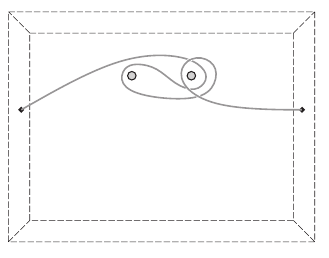
\includegraphics[scale=1]{pics/kartina2}
\caption{Эта картина упадёт если выскочит любой из двух гвоздей.}
\end{figure}

Существуют также некоторые нетопологические решения: например, вы можете сдавить петлю нити между двумя близко расположенными гвоздями, предполагая, что ширина головки гвоздя не намного больше диаметра нити.
Но зачем полагаться на трение, когда можно использовать математику?

\begin{addedbytheeditors}
Попробуйте повесить картину на $n$ гвоздей так, чтобы она упала если выскочит любой из них.
\end{addedbytheeditors}

\subsection*{Дефективный кодовый замок}

Эту шедевр комбинаторики достался мне от Амит Чакрабарти из Дартмута;
он был предложен Восточной Германией для Международную математическую олимпиаду 1988 года.

Задачи такого рода лучше решать геометрически.
Пространство всех возможных комбинаций представляет собой комбинаторный куб $8 \times 8 \times 8$.
Каждый раз, когда мы проверяем комбинацию, мы вычёркиваем все комбинации на трёх ортогональных линиях, проходящих через эту точку.

В так и думать, то вероятно, вы увидите, что лучший способ вычеркнуть все точки в кубе --- брать все тестовые точки в двух противоположных осьмушек $4 \times 4 \times 4$ нашего куба.
Тогда вы придете к решению, эквивалентному описанному ниже.

Проверим все комбинации с числами из $\{1, 2, 3, 4\}$, сумма которых кратна $4$; их шестнадцать, так как если вы выбираете числа на первых двух (или любых двух) циферблатах, число на третьем определяется однозначно.
Теперь попробуем те же комбинации, добавив $(4,4,4)$, то есть, добавив $4$ к каждому из трех чисел;
их ещё $16$, и мы утверждаем, что вместе эти $32$ комбинации вычёркивают все.

Проверка довольно лёгкая.
Правильная комбинация должна иметь либо два (или более) значения из множества $\{1, 2, 3, 4\}$, либо два или более значения из множества $\{5, 6, 7, 8\}$.
В первом случае, существует единственное значение для третьего циферблата (того, чье число может не входить в $\{1, 2, 3, 4\}$), так что полученная тройка среди первых $16$ тестовых комбинаций.
Второй случай аналогичен.

А вот способ Амита (есть и другие) объясняющий, что мы не можем всё вычеркнуть $31$-й или менее тестовыми комбинациями.
Предположим, что $S$ --- это покрытие, и $|S| = 31$.
Пусть $S_i = \{\,(x, y, z) \z\in S : z = i\,\}$ будет $i$-м уровнем $S$.

Рассмотрим три множества:
$A=\{1, 2, 3\}$,
$B = \{4, 5, 6, 7, 8\}$,
и $C \z= \{2, 3, 4, 5, 6, 7, 8\}$.
По крайней мере, один уровень $S$ должен содержать три или меньше точек;
можно считать, что это $S_1$, и $|S_1| = 3$.
(Если $|S_1| \le 2$, то дойти до противоречия ещё проще.)
Точки $S_1$ должны лежать в некотором $3 \times 3 \times 1$ подкубе;
можно считать, что они лежат в $A \times A \times {1}$.

Заметим, что $25$ точек в $B \times B \times \{0\}$ должны быть вычеркнуты точками, не входящими в $S_1$.
Ни какие две из не могут быть вычеркнуты одной точкой в $S$.
Следовательно, $S - S_1$ имеет подмножество $T$ размером $25$, которое лежит в подкубе $B \times B \times C$.
Теперь рассмотрим множество $P = \{\,(x, y, z) : z \in C, (x, y, 1) \notin S_1 , (x, y) \notin B \times B\,\}$.
Легко подсчитать, что $|P| = (64-3-25) \times 7 = 252$.
Точки в $P$ не вычёркиваются $S_1$, и каждая точка в $T$ может вычеркнуть не более $3 + 3 = 6$ точек в $P$. Следовательно, есть по крайней мере $252 - 6 \times 25 = 102$ точки в $P$, которые должны быть вычеркнуты точками в $S - S_1 - T$.

Однако $|S - S_1 - T | = 31 - 3 - 25 = 3$, а каждая из них вычёркивает ровно $22$ точки.
Мы приходим противоречию поскольку $22 \times 3 = 66 \z< 102$.

\subsection*{Альтернативные кости}

Эта задача настолько известна, что у ее решения есть название: "кубики Шихермана".
В колонке Мартина Гарднера от 1978 года [25] или в книге "Пентоны, Ловушки и Криптография" [28] можно узнать об их открытии полковником Джорджем Шихерманом, сейчас проживающим в Уэйсайд, Нью-Джерси.
Единственная пара кубиков Шихермана заключается имеет метки $\{1, 3, 4, 5, 6, 8\}$ и $\{1, 2, 2, 3, 3, 4\}$.

Возможно, вы нашли этот ответ перебором, и это вполне нормально.
Однако есть и другой способ, который иллюстрирует мощный математический инструмент, так называемые \emph{производящие функции}.

Идея в том, чтоб сопоставить кубику многочлен от переменной $x$, в котором коэффициентом при $x^k$ равен числу граней кубика помеченных $k$.
Обычный кубик, например, будет соответствовать многочлену $f(x) = x \z+ x^2 \z+ x^3 \z+ x^4 \z+ x^5 \z+ x^6$.

Ключевое наблюдение заключается в том, что результат броска двух (или более) кубиков представлен произведением их многочленов.
Например, если мы бросаем два обычных кубика, то коэффициент $x^{10}$ в произведении (то есть в $f(x)^2$) есть число способов выбора двух членов из $f(x)$, произведение которых равно $x^{10}$;
это $x^4 \times x^6$, $x^5 \times x^5$ и $x^6 \times x^4$, и они представляют три способа получить сумму $10$.

Следовательно, если $g(x)$ и $h(x)$ --- многочлены, наших кубиков, то $g(x) \times h(x) = f(x)^2$.
Многочлены, как и числа, имеют единственные разложения на простые сомножители;
многочлен $f(x)$ разлагается как $x(x + 1)(x^2 + x + 1)(x^2 - x + 1)$.
Чтобы получить произведение $g(x)$ и $h(x)$ равное $f(x)^2$, нам нужно взять каждый из этих $4$ множителей и добавить по одной его копии в $g(x)$ и в $h(x)$, или же две его копии одному либо другому.
Но есть ограничения: полученные многочлены $g(x)$ и $h(x)$ не могут иметь свободных членов (это бы означало, что некоторые стороны помечены нулём);
также не допускаютая отрицательные коеффициенты;
сумма коеффициентов в каждом из этих многочленов должна равняться 6.


Единственный способ сделать это (кроме $g(x) = h(x) = f(x)$) это
\[g(x)
=
x(x + 1)(x^2 + x + 1)
=
x + 2x^2 + 2x^3 + x^4\]
и
\[h(x)
=
x(x + 1)(x^2 + x + 1)(x^2 - x + 1)^2
=
x + x^3 + x^4 + x^5 + x^6 + x^8,\]
или наоборот.

Мы всё ещё использовали перебор, но таким методом можно решать задачи посложнее.
Во-первых, вы можете изобрести альтернативы для пары восьмигранных кубиков, пронумерованных от $1$ до $8$ (есть три новых способа), или для бросания трех обычных кубиков (множество способов).

Читателям, которые хотят поглубже изучить эту тему, стоит обратиться к отличной статье Джо Галлиана и Дейва Русина [22].


\subsection*{Совпадение монет}

Эту задачу предложил мне Одед Регев, из Техниона, в Израиле.
Сонни и Шер могут выиграть более 2/3 времени, разделив последовательность бросков на блоки по три.
В каждом блоке Шер \emph{сообщает} Сонни, является ли следующий блок в основном орлами или решками;
если первое, Сонни говорит «ООО» в следующем блоке; если второе, то «РРР».

А как Шер передать эту информацию?
Большую часть времени Сонни ошибается (точности) один раз в текущем блоке, и за этот бросок монеты Шер говорит «О», чтобы сообщить ему, что следующий блок в основном состоит из орлов, и «Р» в противном случае.
Для других двух бросков монет в текущей тройке Шер дает правильный ответ (вместе с Сонни), гарантируя две из трёх побед.
Если случится, что Сонни должен угадать все три предположения в текущем раунде, то Шер говорит в один раз --- скажем на третьем броске --- чтобы сообщить, как описано выше, даже если это может стоить им победы в этом броске монеты.
Таким образом, после первого блока Сонни и Шер будут набирать две победы из трех, когда блок состоит из двух орлов и одной решки или двух решек и одного орла.
Когда блок состоит полностью из орлов или полностью из решек (что происходит с вероятностью 1/4), они получают две победы из трех в половине случаев и три из трех в остальной половине.
Всего это позволяет им выигрывать $3/4 \times 2/3 + 1/4 \times 5/6 = 17/24 > 70.8\%$ времени.
Обратите внимание, что даже в наихудшем случае (например, если последовательные орлы и решки выбираются противником, а не случайны), этот метод гарантирует вероятность победы не менее $2/3$.

Оливье Госснер, Пенелопа Эрнандес и Абрахам Нейман [32] доказали, что с более сложными версиями этой схемы Сонни и Шер могут приблизиться к любой доле успеха равной $x$, где $x$ --- единственное решение уравнения
\[-x \log_2 x - (1 - x) \log_2 (1 - x) + (1 - x) \log_2 3 = 1,\]
и лучшего добиться нельзя.
Более того, это утверждение остаётся верным независимо от того, случайны ли броски монеты или нет!
Поскольку это значение $x$ составляет около $0{,}8016$, Сонни и Шер могут на самом деле добиться победы более чем в $80\%$ случаев, даже когда оппонент играет против них.

\subsection*{Имена в коробках}

У этой головоломки короткая, но увлекательная история.
Она придумана датским компьютерным ученым Петером Бро Милтерсеном, версия появилась в статье, написанной им и Анной Галь [21], получившей приз???.
Однако Милтерсен не знал, что есть решение, пока его коллега Свен Скиум не указал ему на это во время обеда.
В конечном итоге головоломка дошла до меня (в несколько более сложной форме, чем здесь) через Дорит Ахаронов.

Чтобы её решить, заключенные должны сначала договориться о случайном соответствии ящиков со своими именами.
(Это сделает невозможным разложить имена в ящиках таким образом, чтобы помешать протоколу, описанному ниже.)
Попадая в комнату, каждый заключенный проверяет свой собственный ящик (то есть ящик, с которому соответсвует его имя).
Затем он заглядывает в ящик, соответствующий имени, которое он только что нашел, а затем в ящик, соответствующий имени, найденному во втором ящике, и так далее, пока он не найдет свое собственное имя или не откроет 50 ящиков.

Вот такая стратегия, а почему она работает?
Ну хорошо, процесс, который назначает владельцу ящика имя, найденное в его ящике, представляет собой перестановку из 100 имен, выбранную равномерно случайным образом из набора всех таких перестановок.
Каждый заключенный идёт по циклу перестановки, начиная со своего ящика, и, если цикл не длиннее 50, он находит своё имя.
Если перестановка не имеет циклов длиной 50 и выше, то это сработает для всех, и заключенные будут спасены.

Вероятность того, что равномерно случайная перестановка чисел от $1$ до $2n$ не содержит ни одного цикла длиной более $n$, по крайней мере, $1$ минус натуральный логарифм от $2$, что составляет около $30,6853\%$.
Чтобы увидеть это, пусть $n < k \le 2n$ и посчитаем перестановки, имеющие цикл длиной ровно $k$.
Есть $k$ способов выбрать записи в цикле $C$, $(k - 1)!$ способов упорядочить их и $(2n - k)!$ способов перестановки остальных; произведение этих чисел равно $(2n)!/k$.
Поскольку в данной перестановке может существовать не более одного $k$-цикла, вероятность того, что такой существует, точно равна $1/k$.
Отсюда следует, что вероятность отсутствия длинного цикла равна
\[1-\frac{1}{n}-\frac{1}{n+1}-\dots-\frac{1}{2n}=1-H_{2n}-H_n\]
где $H_m$ --- сумма обратных чисел первых $m$ положительных целых чисел, что приблизительно равно $\ln m$.
Таким образом, наша вероятность будет близка к $1 - \ln 2n + \ln n = 1 - \ln 2$ на самом длеле всегда чуть больше этого значения.
Для $n = 50$ мы получаем, что заключенные выживают с вероятностью $31,1827821\%$.
Недавно Юджин  Кертин и Макс Варшауэр [13] показали, что это решение нельзя улучшить.

Ламберт Брайт и Рори Ларсон, а также независимо Ричард Стэнли из Массачусетского технологического института, предложили следующую вариацию.
Предположим, что каждый заключенный должен заглянуть в \emph{не менее} чем 50 ящиков, и требование для выживания заключается в том, чтобы каждый заключенный \emph{не} нашёл собственное имя?
Несмотря на то, что цель полностью противоположна, кажется, что у заключенных не могут поступить иначе, кроме как следовать точно той же стратегии.
Здесь, однако, они выживают только в том случае, если каждый цикл состоит более чем из $50$ ящиков, что может произойти только в случае наличия одного большого цикла --- для чего их шансы составляют ровно $1$ к $100$.
Не сильно обнадёживает, но всё же намного лучше, чем $1$ к $2^{100}$.

Заметим, что у заключённых будут те же шансы если каждому потребуется заглянуть в $99$ ящиков --- снова они следуют стратегии и выигрывают только тогда, когда случайная перестановка имеет только один большой цикл.
В этом случае сразу очевидно, что лучшей стратегии нет, потому что у самого первого заключенного, несмотря на все его действия, имеет максимум $1\%$ вероятности избежать своего собственного имени.
Забавно, что, следуя этой стратегии, если повезло первому заключенному, то автоматически везёт всем остальным!
